\newpage
%%%%%%%%%%%%%%%%%%%%%%%%%%%%%%%%%%%%%%%%%%%%%%%

\section{Markets}

{\it This lecture applies the ideas developed in the first two lectures to markets. 

We set up a simple portfolio selection problem in a market of two assets: one risky, like shares; and the other riskless, like a bank deposit. We ask how an investor should best allocate his money between the two assets, which we phrase in terms of his leverage. We review the classical approach, which can't answer this question without additional information about the investor's risk preferences. We then use the decision theory we've developed so far to answer the question unambiguously, by deriving the optimal leverage which maximises the investment's time-average growth rate.

Next, we consider what this objectively defined optimal leverage might mean for financial markets themselves. If all the participants in a market aim for the same optimal leverage, does this constrain the prices and price fluctuations that emerge from their trading? We argue that it does, and we quantify how. Our treatment of the problem resolves the so-called equity premium puzzle (and the price volatility puzzle), and it provides a natural framework for setting central-bank interest rates.
We test our predictions using data collected from the American and German stock markets as well as Bitcoin.
}

\newpage


%%%%%%%%%%%%%%%%%%%%%%%%%%%%%%%%%%%%%%%%%%%%%%%
\subsection{Optimal leverage}

%%%%%%%%%%%%%%%%%%%%%%%%%%%%%%%%%%%%%%%%%%%%%%%
\subsubsection{A model market}
We consider assets whose values follow multiplicative dynamics, which we will model using \GBM. In general, an amount $\x$ invested in such an asset evolves according to the \SDE,
\be
d\x = \x(\gmu d\t + \gsigma d\gW),
\elabel{sde_gbm}
\ee
where $\gmu$ is the drift and $\gsigma$ is the volatility. By now we are very familiar with this equation and how to solve it.

To keep things simple, we imagine a market of two assets. One asset is riskless: the growth in its value is known deterministically and comes with a cast-iron guarantee.\footnote{Such guarantees are easy to offer in a model. In the real world, one should be very suspicious of anything that comes with a ``cast-iron guarantee''.} This might correspond in reality to a bank deposit. The other asset is risky: there is uncertainty over what its value will be in the future. This might correspond to a share in a company or a collection of shares in different companies. We will think of it simply as stock.

An amount $\xzero$ invested in the riskless asset evolves according to
\be
d\xzero = \xzero \mur d\t.
\elabel{sde_0}
\ee
$\mur$ is the riskless drift, known in finance as the riskless rate of return.\footnote{In general we will eschew financial terminology for rates. Economics has failed to define them clearly, with the result that different quantities, like $\gt$ and $\gex$, are often conflated. The definitions developed in these lectures are aimed at avoiding such confusion.} There is no volatility term. In effect, we have set $\gsigma=0$. We know with certainty what $\xzero$ will be at any point in the future: 
\be
\xzero(\tn+\Dt) = \xzero(\tn)\exp(\mur\Dt).
\elabel{sde_0_soln}
\ee

An amount $\xone$ invested in the risky asset evolves according to
\be
d\xone = \xone ( \mus d\t + \sigmas d\gW ),
\elabel{sde_1}
\ee
where $\mus>\mur$ is the risky drift and $\sigmas>0$ is the volatility (the subscript s stands for stock). $\mus$ is also known in finance as the expected return.\footnote{Probably because it's the growth rate of the expected value, see \eref{exp_ret}.} This equation has solution
\be
\xone(\tn+\Dt) = \xone(\tn)\exp\left[\left(\mus -\frac{\sigmas^2}{2}\right)\Dt + \sigmas \gW(\Dt)\right],
\elabel{sde_1_soln}
\ee
which is a random variable.

The difference
\be
\mue=\mus-\mur
\elabel{def_mue}
\ee
is known variously as the excess return, the risk premium, and in stock markets as the equity premium. We will refer to it simply as the excess drift. It will be a very important quantity in later discussions. For the moment we can think of it as compensation for accepting the uncertain outcome of \eref{sde_1_soln} instead of the guaranteed result of \eref{sde_0_soln}.

%%%%%%%%%%%%%%%%%%%%%%%%%%%%%%%%%%%%%%%%%%%%%%%
\subsubsection{Leverage}
Let's turn to the concept of leverage. Imagine a very simple portfolio of value $\xl$, out of which $\l \xl$ is invested in stock and the remainder, $(1-\l)\xl$, is put in the bank. $\l$ is known as the leverage. It is the fraction of the total investment assigned to the risky asset. $\l=0$ corresponds to a portfolio consisting only of bank deposits. $\l=1$ corresponds to a portfolio only of stock.

You would be forgiven for thinking that prudence dictates $0\leq\l\leq1$, \ie that we invest some of our money in stock and keep the rest in the bank. However, the financial markets have found all sorts of exciting ways for us to invest almost any amount in an asset. For example, we can make $\l>1$ by borrowing money from the bank to buy more stock than we could have bought with only our own money.\footnote{This doesn't immediately affect the portfolio's value. The bank loan constitutes a negative investment in the riskless asset, whose value cancels the value of the stock we bought with it. Of course, the change in the portfolio's composition will affect its future value.} We can even make $\l<0$ by borrowing stock (a negative investment in the risky asset), selling it, and putting the money raised in the bank. In the financial world this practice is called short selling.

Each investment in our portfolio experiences the same relative fluctuations as the asset in which it has been made. The overall fluctuation in the portfolio's value is, therefore,
\be
d\xl = (1-\l)\xl \frac{d\xzero}{\xzero} + \l \xl \frac{d\xone}{\xone}.
\ee
Substituting in \eref{sde_0} and \eref{sde_1} gives the \SDE for a leveraged investment in the risky asset,
\be
d\xl = \xl [ (\mur + \l\mue) d\t + \l\sigmas d\gW ],
\elabel{sde_l}
\ee
with solution,
\be
\xl(\tn+\Dt) = \xl(\tn)\exp\left[\left(\mur+\l\mue-\frac{\l^2\sigmas^2}{2}\right)\Dt+\l\sigmas \gW(\Dt)\right].
\elabel{sde_l_soln}
\ee
We can now see why we labelled investments in the riskless and risky assets by $\xzero$ and $\xone$: when $\l=0$, $\xl$ follows the same evolution as $\xzero$; and when $\l=1$, it evolves as $\xone$.

In our model $\l$, once chosen, is held constant over time. This means that our model portfolio must be continuously rebalanced to ensure that the ratio of stock to total investment stays fixed at $\l$. For example, imagine our stock investment fluctuates down over a short time-step, while our bank deposit accrues a little interest. Immediately we have slightly less than $\l$ of the portfolio's value in stock, and slightly more than $1-\l$ of its value in the bank. To return the leverage to $\l$, we need to withdraw some money from the bank and use it to buy more stock. In \eref{sde_l} we are imagining that this happens continuously.\footnote{In reality, of course, that's not possible. We could try to get close by rebalancing frequently. However, every time we buy or sell an asset in a real market, we pay transaction costs, such as broker's fees and transaction taxes. This means that frequent rebalancing in the real world can be costly.}

%%%%%%%%%%%%%%%%%%%%%%%%%%%%%%%%%%%%%%%%%%%%%%%
\subsubsection{Portfolio theory\seclabel{pf_theory}}
Our simple model portfolio parametrised by $\l$ allows us to ask the
\begin{keypts}{Question:}
What is the optimal value of $\l$?
\end{keypts}
This is similar to choosing between gambles, for which we have already developed a decision theory. The main difference is that we are now choosing from a continuum of gambles, each characterised by a value of $\l$, whereas previously we were choosing between discrete gambles. The principle, however, is the same: we will maximise the time-average growth rate of our investment.

Before we do this, let's review the classical treatment of the problem so that we appreciate the wider context. Intuitively, people understand there is some kind of trade-off between risk and reward. In our model of a generic multiplicative asset, \eref{sde_gbm}, we could use $\gsigma$ as a proxy for risk and $\gmu$ as a proxy for reward. Ideally we want an investment with large $\gmu$ and small $\gsigma$, but we also acknowledge the rule-of-thumb that assets with larger $\gmu$ tend to have larger $\gsigma$.\footnote{A ``no such thing as a free lunch'' type of rule.} This is why we model our risky asset as having a positive excess return, $\mue>0$, over the riskless asset.

Intuition will only take us so far. A rigorous treatment of the portfolio selection problem was first attempted by Markowitz in 1952~\cite{Markowitz1952}. He suggested defining a portfolio with parameters $(\gsigma_i, \gmu_i)$ as efficient if there exists no rival portfolio with parameters $(\gsigma_j, \gmu_j)$ with $\gmu_j\geq\gmu_i$ and $\gsigma_j\leq\gsigma_i$.
% AA: simplified definition of Markwoitz-efficient for clarity at tiny cost of rigour
%for which at least one of the following statements is true:
%\begin{enumerate}
%\item $\gmu_j>\gmu_i$ and $\gsigma_j\leq\gsigma_i$;
%\item $\gsigma_j<\gsigma_i$ and $\gmu_j\geq\gmu_i$.
%\end{enumerate}
%In other words, if the rival portfolio has higher $\gmu$, it had better have higher $\gsigma$; or if it has lower $\gsigma$, it had better have lower $\gmu$.
Markowitz argued that it is unwise to invest in a portfolio which is not efficient.

In our problem, we are comparing portfolios with parameters $(\l\sigmas, \mur+\l\mue)$. These lie on a straight line in the $(\gsigma, \gmu)$-plane,\footnote{Derived by eliminating $\l$ from the equations $\gmu=\mur+\l\mue$ and $\gsigma=\l\sigmas$.}
\be
\gmu = \mur + \left(\frac{\mue}{\sigmas}\right)\gsigma,
\elabel{frontier}
\ee
shown schematically in \fref{markowitz}.
\begin{figure}
\centering
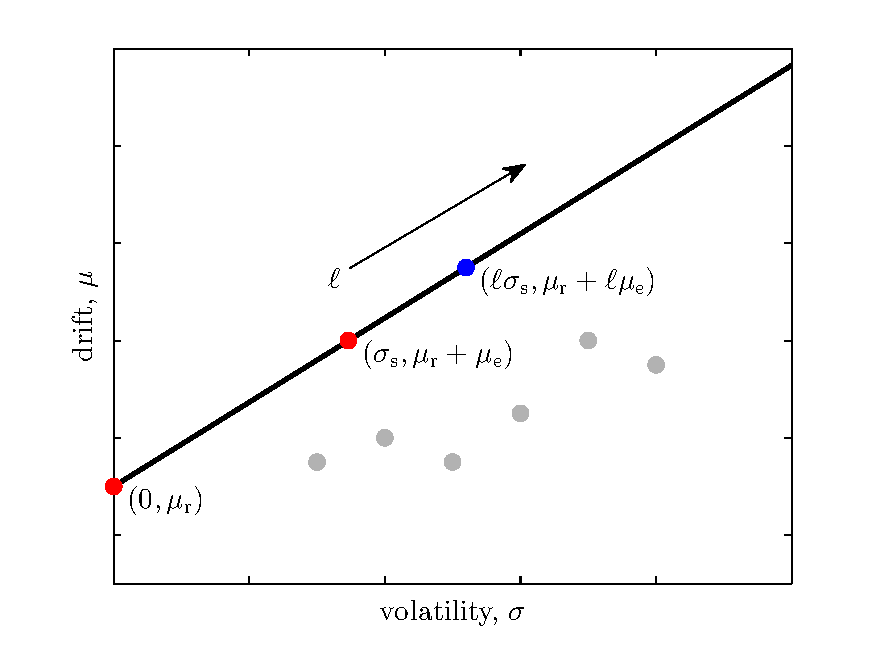
\includegraphics[width=\textwidth]{./chapter_4/figs/markowitz.pdf}
\caption{The Markowitz portfolio selection picture. The red dots are the locations in the $(\gsigma,\gmu)$-plane of portfolios containing only the riskless (left) or risky (right) asset. The blue dot is one possible leveraged portfolio, in this case with $\l>1$. All possible leveraged portfolios lie on the black line, \eref{frontier}. The grey dots are hypothetical alternative portfolios, containing different assets excluded from our simple portfolio problem. Their location below and to the right of the black line makes them inefficient under the Markowitz scheme.\flabel{markowitz}}
\end{figure}
Under Markowitz's classification, all of the leveraged portfolios on this line are efficient.\footnote{Indeed, in finance this line is called the efficient frontier.} Therefore, any leverage we choose gives a portfolio in which we are not counselled against investing. This does not help answer our question. By itself, Markowitz's approach is agnostic to leverage: it requires additional information to distinguish between portfolios. Markowitz was aware of this limitation and argued that the optimal portfolio could be identified by considering the investor's risk preferences.\footnote{``The proper choice among portfolios depends on the willingness and ability of the investor to assume risk.''~\cite{Markowitz1991}.} Typically this is modelled by the introduction of a utility function, with which approach we are now familiar.

%%%%%%%%%%%%%%%%%%%%%%%%%%%%%%%%%%%%%%%%%%%%%%%
\subsubsection{Sharpe ratio\seclabel{sharpe}}
The Sharpe ratio~\cite{Sharpe1966} for an asset with drift $\gmu$ and volatility $\gsigma$ is defined as
\be
\Sharpe\equiv\frac{\gmu-\mur}{\gsigma}
\elabel{def_sharpe}
\ee
It is the gradient of the straight line in the $(\gsigma, \gmu)$-plane which passes through the riskless asset and the asset in question. $\Sharpe$ is often used as a convenient shorthand for applying Markowitz's ideas, since choosing the portfolio with the highest $\Sharpe$ from the set of available portfolios is equivalent to choosing an efficient portfolio. In our scenario, however, we can immediately see why it sheds no light. All of our leveraged portfolios lie on the same line, \eref{frontier}, and so all of them have the same Sharpe ratio, which is simply the line's gradient:
\be
\Sharpe_\l = \frac{\mue}{\sigmas}.
\elabel{sharpe_l}
\ee
This is insensitive to the leverage $\l$, resulting in the same non-advice as the Markowitz approach. Sharpe also suggested considering risk preferences to resolve the optimal portfolio.\footnote{``The investor's task is to select from among the efficient portfolios the one that he considers most desirable, based on his particular feelings regarding risk and expected return.''~\cite{Sharpe1966}.}

%%%%%%%%%%%%%%%%%%%%%%%%%%%%%%%%%%%%%%%%%%%%%%%
\subsubsection{Expected return\seclabel{exp_ret}}
We noted previously that the growth rate of the expected value of the risky asset is the risky drift, $\mus$, also known as the expected return. This is because
\be
\ave{\xone(\tn+\Dt)} = \ave{\xone(\tn)}\exp(\mus \Dt),
\elabel{exp_ret}
\ee
which, as a multiplicative process, has growth rate
\be
\gm(\ave{\xone}) = \frac{\D\ln\ave{\xone}}{\Dt} = \mus.
\ee
It follows immediately from comparison of \eref{sde_1} and \eref{sde_l} that the expected value of the leveraged portfolio grows at
\be
\gm(\ave{\xl}) = \mur+\l\mue.
\elabel{exp_ret_l}
\ee
This illustrates why a portfolio theory which is insensitive to leverage, such as that of Markowitz and Sharpe\footnote{Both recipients of the 1990 Alfred Nobel Memorial Prize in Economic Sciences.}, is potentially dangerous. If any leverage is admissible, then an investor misguidedly seeking to maximise his expected return in \eref{exp_ret_l} would maximise his leverage, $\l\to\infty$. This, as we will shortly see, would almost surely ruin him.

%%%%%%%%%%%%%%%%%%%%%%%%%%%%%%%%%%%%%%%%%%%%%%%
\subsubsection{Growth rate maximisation}
We now understand the classical approach, as applied to a very simple portfolio problem, and we are aware of its limitations. What does our own decision theory have to say?

The time-average growth rate of the leveraged portfolio is
\be
\gtm(\l) \equiv \lim_{\Dt\to\infty} \left\{ \gm(\xl,\Dt) \right\} = \lim_{\Dt\to\infty} \left\{ \frac{\D\ln \xl}{\Dt} \right\}.
\ee
This will depend on $\l$. Inserting the expression for $\xl$ in \eref{sde_l_soln} gives
\be
\gtm(\l) = \lim_{\Dt\to\infty} \left\{ \frac{1}{\Dt} \left[ \left(\mur + \l\mue - \frac{\l^2\sigmas^2}{2}\right)\Dt + \l\sigmas \gW(\Dt) \right] \right\},
\elabel{g_l_noisy}
\ee
which, since $\gW(\Dt)/\Dt\sim\Dt^{-1/2}\to0$ as $\Dt\to\infty$, converges to
\be
\boxed{\; \gtm(\l) = \mur + \l\mue - \frac{\l^2\sigmas^2}{2}. \;}
\elabel{g_l_quadratic}
\ee
This is a quadratic in $\l$ with an unambiguous maximum\footnote{Derived, for example, by setting $\frac{d\gtm}{d\l}=0$.} at
\be
\boxed{\; \lopt = \frac{\mue}{\sigmas^2}. \;}
\elabel{lopt}
\ee
$\lopt$ is the optimal leverage which defines the portfolio with the highest time-average growth rate. Classical theory is indifferent to where on the line in \fref{markowitz} we choose to be. Our decision theory, however, selects a particular point on that line,\footnote{Subsequently Markowitz became aware of this point, which he called the ``Kelly-Latan\'{e}'' point in~\cite{Markowitz1976}, referring to~\cite{Kelly1956,Latane1959}.} which answers the question we posed at the start of \secref{pf_theory}. This is the key result. We note that it requires no additional knowledge to the parameters $\mur$, $\mus$, and $\sigmas$ of the two assets in our market. In particular, it is defined objectively, with no reference to idiosyncrasies of the investor (other than that we assume him to be a time-average growth rate maximiser).

\eref{g_l_quadratic} gives the time-average growth rate along the efficient frontier, where all of our leveraged portfolios lie. In fact, it's easy to calculate the growth rate for any point in the $(\gsigma,\gmu)$-plane: it is simply $\gmu-\gsigma^2/2$. Overlaying the Markowitz picture in \fref{markowitz} on the growth rate landscape is illuminating. In effect, it adds the information missing from the classical model, which was needed to distinguish between portfolios. This is shown in \fref{markowitz_peters}.
\begin{figure}
\centering
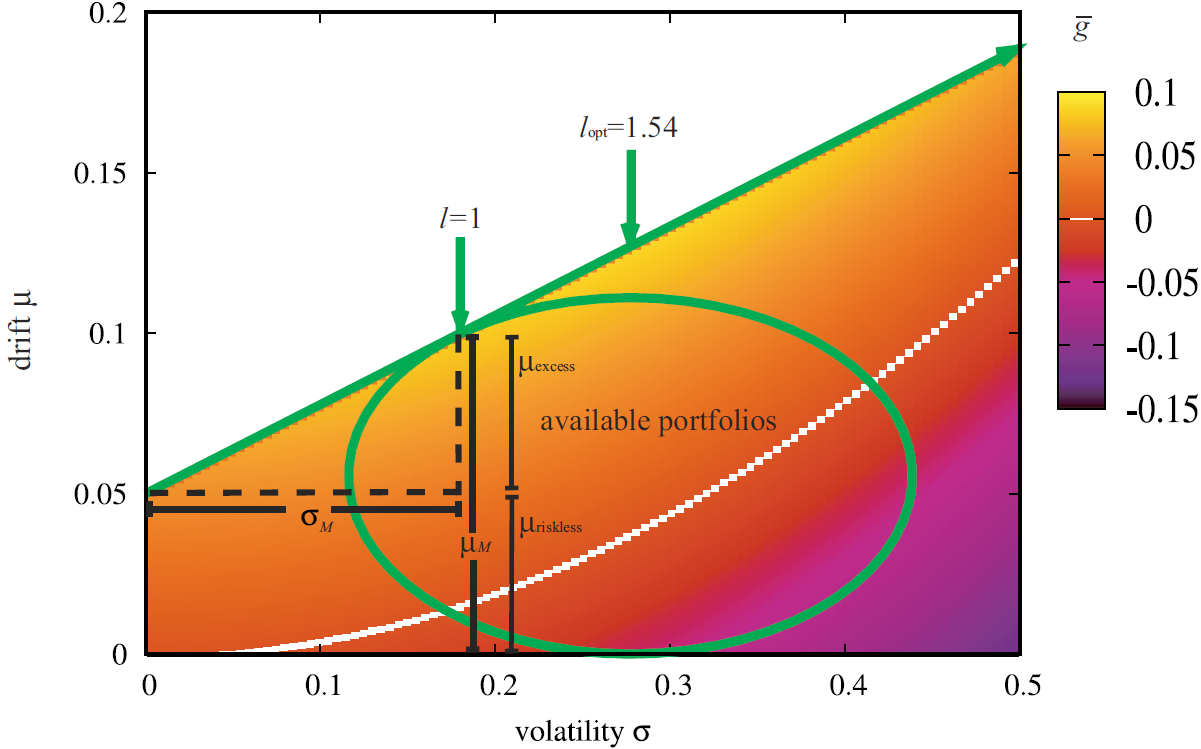
\includegraphics[width=\textwidth]{./chapter_4/figs/markowitz_peters.png}
\caption{The augmented portfolio selection picture. The Markowitz picture is shown in green, with our model leveraged portfolios on the straight line (the efficient frontier) and hypothetical alternative portfolios within the ellipse (analogous to the grey dots in \fref{markowitz}). This is overlaid on a colour plot of the time-average growth rate, $\gt$. The optimal leverage, $\lopt\approx1.54$, is marked at the location of the highest $\gt$ on the efficient frontier. Portfolios on the white curve have $\gt=0$. Eventually this will intersect the efficient frontier, at which point applying more leverage will produce a portfolio with negative long-run growth. Parameters are $\mur=\mue=0.05$ per unit time and $\sigmas=0.18$ per square root time (denoted by $\gmu_\text{riskless}$, $\gmu_\text{excess}$, and $\gsigma_\text{M}$ in the figure). Adapted from~\cite{Peters2011a}.\flabel{markowitz_peters}}
\end{figure}

That \eref{g_l_quadratic} defines an inverted parabola means that, even on the efficient frontier, there exist portfolios with $\gtm(\l) < 0$. These occur for $\l<\lm$ and $\l>\lp$, where
\be 
\lpm \equiv \lopt \pm \sqrt{\lopt^2 + \frac{2\mur}{\sigmas^2}}.
\ee
This confirms our assertion at the end of \secref{exp_ret}, that an investor maximising his leverage in either direction will, if he is able to apply enough leverage, subject his wealth to negative time-average growth. Indeed, if his leveraging ability is unlimited, he will find to his horror what is easily seen in \eref{g_l_quadratic}, that $\gtm(\l)$ diverges negatively as $\l\to\pm\infty$.

%%%%%%%%%%%%%%%%%%%%%%%%%%%%%%%%%%%%%%%%%%%%%%%
\subsection{Stochastic market efficiency\seclabel{Stochastic}}


%%%%%%%%%%%%%%%%%%%%%%%%%%%%%%%%%%%%%%%%%%%%%%%
\subsubsection{A fundamental measure\seclabel{fundamental}}
Aside from being insensitive to leverage, the Sharpe ratio, $\Sharpe=\mue/\sigmas$, is a dimensionful quantity. Its unit is $(\text{time unit})^{-1/2}$. This means that its numerical value is arbitrary (since it depends on the choice of time unit) and tells us nothing fundamental about the system under study. For example, a portfolio with $\Sharpe=5$ per square root of one year has $\Sharpe=5(365)^{-1/2}\approx0.26$ per square root of one day. Same portfolio, different numbers.

The optimal leverage, $\lopt=\mue/\sigmas^2$, which differs from the Sharpe ratio by a factor of $1/\sigmas$, is a dimensionless quantity. Therefore, its numerical value does not depend on choice of units and has the potential to carry fundamental information about the system.\footnote{See Barenblatt's modern classic on scaling~\cite{Barenblatt2003}.} We could view $\lopt$ as the fundamental measure of a portfolio's quality, similarly to how $\Sharpe$ is viewed in the classical picture. A portfolio with a high optimal leverage must represent a good investment opportunity to justify such a large commitment of the investor's funds.

However, the significance of $\lopt$ runs deeper than this. The portfolio to which $\lopt$ refers is that which optimally allocates money between the risky and riskless assets in our model market. Therefore, it tells us much about conditions in that market and, by extension, in the wider model economy. A high $\lopt$ indicates an economic environment in which investors are incentivised to take risks. A low or negative $\lopt$ indicates the converse. This raises a tantalising
\begin{keypts}{Question:}
Are there any special numerical values of $\lopt$ which describe different market regimes, or to which markets are attracted?
\end{keypts}

%%%%%%%%%%%%%%%%%%%%%%%%%%%%%%%%%%%%%%%%%%%%%%%
\subsubsection{Relaxing the model}
Our model market contains assets whose prices follow \GBM with constant drift and volatility parameters.\footnote{A tautology, since \eref{sde_gbm} only describes a \GBM if $\gmu$ and $\gsigma$ are constant in time.} Once specified, $\mur$, $\mus$, and $\sigmas$ are static and, therefore, so is $\lopt$. This limits the extent to which we can explore the question, since we cannot consider changes in $\lopt$. To make progress we need to relax the model. We must consider which parts of the model are relevant to the question, and which parts can be discarded without grave loss.

The \GBM-based model is useful because it motivates the idea of an objectively optimal leverage which maximises the growth of an investment over time. It also provides an expression for $\lopt$ in terms of parameters which, in essence, describe the market conditions under which prices fluctuate. These parameters have correspondences with quantities we can measure in real markets. All of this is useful.

However, the real markets in which we are ultimately interested contain assets whose prices do not follow \GBM (because nothing in nature\footnote{We consider markets to be part of nature and appropriate subjects of scientific study.} truly does). In particular, real market conditions are not static. They change over time, albeit on a longer time scale than that of the price fluctuations. In this context, the model assumption of constant $\mur$, $\mus$, and $\sigmas$ is restrictive and unhelpful. We will relax it and imagine a less constrained model market in which these parameters, and therefore $\lopt$, are allowed to vary slowly. We will not build a detailed mathematical formulation of this, but instead use the idea to run some simple thought experiments.

%%%%%%%%%%%%%%%%%%%%%%%%%%%%%%%%%%%%%%%%%%%%%%%
\subsubsection{Efficiency}
One way of approaching a question like this is to invoke the concept of efficiency. In economics this has a specific meaning in the context of financial markets, which we will mention imminently. In general terms, an efficient system is one which is already well optimised and whose performance cannot be improved upon by simple actions. For example, a refrigerator is efficient if it maintains a cool internal environment while consuming little electrical power and emitting little noise. Similarly, Markowitz's portfolios were efficient because the investor could do no better than to choose one of them. 

The ``efficient market hypothesis'' of classical economics treats markets as efficient processors of information. It claims that the price of an asset in an efficient market reflects all of the publicly available information about it. The corollary is that no market participant, without access to privileged information, can consistently beat the market simply by choosing the prices at which he buys and sells assets. We shall refer to this hypothesis as ordinary efficiency.\footnote{This is not the most precise hypothesis ever hypothesised. What does it mean for a price to ``reflect'' information? Presumably this involves some comparison between the observed price of the asset and its true value contingent on that information. But only the former is observable, while the latter evades clear definition. Similarly, what does it mean to ``beat the market''? Presumably something to do with achieving a higher growth rate than a general, na\"{i}ve investment in the overall market. But what investment, exactly? We will leave these legitimate questions unanswered here, since our focus is a different form of market efficiency. The interested reader can consult the comprehensive review in~\cite{Sewell2011}.}

We will consider a different sort of efficiency, where we think not about the price at which assets are bought and sold in our model market, but instead about the leverage that is applied to them. Let's run a thought experiment.

\begin{thoughtex}{efficiency under leverage}
Imagine that $\lopt>1$ in our model market. This would mean that the simple strategy of borrowing money to buy stock will achieve faster long-run growth than buying stock only with our own money. If we associate putting all our money in stock, $\l=1$, with an investment in the market, then it would be a trivial matter for us to beat the market (by doing nothing more sophisticated than investing borrowed money).

Similarly, imagine that $\lopt<1$. In this scenario, the market could again be beaten very easily by leaving some money in the bank (and, if $\lopt<0$, by short selling).
\end{thoughtex}

It would strain language to consider our market efficient if consistent outperformance were so straightforward to achieve. This suggests a different, fluctuations-based notion of market efficiency, which we call stochastic efficiency. We claim that it is impossible for a market participant without privileged information to beat a stochastically efficient market simply by choosing the \textit{amount} he invests in stock, \ie by choosing his leverage.\footnote{This resembles ordinary efficiency except that we have replaced price by amount.} Therefore, we make the following

\begin{keypts}{Hypothesis: stochastic market efficiency}
Real markets self-organise such that
\be
\boxed{\; \lopt = 1 \;}
\elabel{sme_strong}
\ee
is an attractive point for their stochastic properties.
\end{keypts}

These stochastic properties are represented by $\mur$, $\mus$, and $\sigmas$ in the relaxed model, in which we permit dynamic adjustment of their values. We call this the strong form of the hypothesis, since it makes a very precise prediction about the attractive value for $\lopt$.

%%%%%%%%%%%%%%%%%%%%%%%%%%%%%%%%%%%%%%%%%%%%%%%
\subsubsection{Stability}
Another approach to the question in \secref{fundamental}, whose style owes more to physics than economics, is to consider the stability of the system under study (here, the market) and how this depends on the value of the measure in question (here, $\lopt$). Systems which are stable tend to persist over long time scales and are usually what we observe in nature. Unstable systems tend to last for shorter times,\footnote{We use the comparative ``shorter'' here. This does not mean short. It is quite possible for an unstable system to remain in flux for a long time in human terms, perhaps giving the illusion of stability. Indeed, much of classical economic theory is predicated on the idea that economies are at or close to equilibrium, \ie stable. We would argue that economies are fundamentally far-from-equilibrium systems and must be modelled as such, even if their dynamics unfold over time scales much longer than our day-to-day affairs.} so we observe them less frequently. With this in mind, let's think about the logic of different values of $\lopt$.

\begin{thoughtex}{stability under leverage}
Imagine that $\lopt>1$ in our relaxed model. Since it is an objectively optimal leverage which does not depend on investor idiosyncrasies, this means that \textit{everyone} in the market should want to borrow money to buy stock. But, if that's true, who's going to lend the money and who's going to sell the stock?

Similarly, imagine that $\lopt<0$. This means that \textit{everyone} should want to borrow stock and sell it for cash. But, if that's true, who's going to lend the stock and who's going to relinquish their cash to buy it?

Unless there are enough market participants disinterested in their time-average growth rate to take the unfavourable sides of these deals -- which in our model we will assume there aren't -- then neither of these situations is globally stable. It's hard to imagine them persisting for long before trading activity causes one or more of the market parameters to change, returning $\lopt$ to a stable value.
\end{thoughtex}

This thought experiment suggests that we could observe markets with $0\leq\lopt\leq1$. This probably doesn't correspond to a macroeconomically desirable state, but it wouldn't be unstable purely from the leverage point of view. Whether real markets spend significant time in this phase is difficult to tell. Realistic optimal leverage depends significantly on such things as trading costs, access to credit and risky assets in lending programs, infrastructure and technology. All of these factors differ among market participants. They suggest that measuring optimal leverage in the simplest way -- using market prices only and assuming zero trading costs -- will produce an over-estimate, compared to the value experienced by real market participants who incur realistic costs.

The dynamical adjustment, or self-organisation, of the market parameters takes place through the trading activity of market participants. In particular, this creates feedback loops, which cause prices and fluctuation amplitudes to change, returning $\lopt$ to a stable value whenever it strays. To be truly convincing, we should propose plausible trading mechanisms through which these feedback loops arise. We do this in~\cite{PetersAdamou2013}. Since they involve details about how trading takes place in financial markets (in which we assume the typical attendee of these lectures is disinterested) we shall not rehearse them here. The primary drivers of our hypothesis are the efficiency and stability arguments we've just made.

Furthermore, there are additional reasons why we would favour the strong form of the hypothesis over long time scales. The main one is that an economy in which $\lopt$ is close to, or even less than, zero gives people no incentive to invest in productive business activity. Such an economy would appear paralysed, resembling perhaps those periods in history to which economists refer as depressions. We'd like to think that economies are not systematically attracted to such states. The other reasons are more technical, to do with the different interest rates accrued on deposits and loans, and the costs associated with buying and selling assets. These are described in~\cite{PetersAdamou2013} and lead to a refined
\begin{keypts}{Hypothesis: stochastic market efficiency (refined)}
On sufficiently long time scales, $\lopt=1$ is a strong attractor for the stochastic properties of real markets. Deviations from this attractor over shorter time scales are likely to be confined to the range $0\leq\lopt\leq1$.
\end{keypts}


\subsubsection{Prediction accuracy\seclabel{Prediction_accuracy}}
When we simply use observed price changes to compute changes in invested wealth, we will overestimate optimal leverage. Denoting an estimate from real data of $\lopt$ by $\loptc$, we will  have $\loptc>\lopt$. This is because real investments incur transaction costs and other costs associated with leveraging. We therefore expect na\"ively measured values to be a little too big, $\loptc>1$. 

Ignoring these effects for the moment, we can predict how close we expect observed optimal leverage to be to its predicted value, 1, when we estimate it from a finite time series. Even assuming that our theory is correct and 
$\lopt$ is attracted to a particular value, we expect random
deviations from it to increase as the time series gets shorter. To take an extreme example, with daily data, the observed optimal leverage over a
window of one day does not exist. Either $\loptc \to+\infty$ if the
risky return beats the deposit rate on that day; or $\loptc \to -\infty$ if
deposits beat the risky asset. Indeed, the magnitude of the observed
optimal leverage will diverge for any window over which the daily
risky returns are either all greater than, or all less than, the daily returns on federal
funds. This is unlikely for windows of months or years but using daily data it happens
commonly over windows of days or weeks. Even without this
divergence, shorter windows are more likely to result in larger
positive and negative optimal leverages because relative fluctuations
are larger over shorter time scales.

To quantify this idea we compute $\gm(\xl,\Dt)$, \ie the time-average growth rate after a finite
time $\Dt$. That's simply the expression on the \RHS of \eref{g_l_noisy} without taking the $\Dt\to\infty$ limit:
\begin{equation}
\gm(\xl,\Dt) =
\mur + \l\mue - \frac{(\l\sigmas)^2}{2} + \frac{\l\sigmas \gW(\Dt)}{\Dt}
%
%\murm+\lm\muem-\frac{(\lm\sigmam)^2}{2}+\frac{\lm\sigmam W(\Dt)}{\Dt}.
\end{equation}
Maximizing this generates a noisy estimate for the optimal leverage over a window of length $\Dt$:
\begin{equation}
\loptc(\Dt, N=1) = \lopt + \frac{\gW(\Dt)}{\sigmas \Dt}.
\end{equation}
Thus, in the model, optimal leverage for finite time series is
normally distributed with mean $\lopt$ and standard deviation
\begin{equation}
\text{stdev}(\loptc(\Dt)) = \frac{1}{\sigmas \Dt^{1/2}}.
\elabel{variance}
\end{equation}
We will use this quantity as the standard error for the prediction $\loptc=1$. 


\subsection{Applications of stochastic market efficiency\seclabel{applications}}

\subsubsection{A theory of noise -- the silliness of price discovery\seclabel{a_theory}}
According to leverage efficiency, prices of risky assets must fluctuate if an excess drift exists, $\mue>0$, simply because the market would otherwise become unstable. But, if price fluctuations are necessary for stability, then the intellectual basis for price efficiency -- that changes in price are driven by the arrival of new economic information --  cannot be the whole truth. At least some component of observed fluctuations must be driven by the leverage feedbacks described in section~\secref{Stochastic}, which enforce leverage efficiency and which have little to do with information arrival.

\cite{Black1986} differentiated between information-based and other types of price fluctuation, referring to the latter as ``noise'' and regarding it as a symptom of inaccurate information and market {\it in}-efficiency. However, substituting $\lopt=1$ in \eref{lopt} yields 
\be
\elabel{noise}
\left(\sigmas\right)^2=\mue.
\ee
Purely based on leverage efficiency, prices must fluctuate, and we can even quantify by how much. An asset whose expectation value grows faster than than of the riskless asset must fluctuate; otherwise systemic stability will be undermined.
This is a radical departure from conventional thinking, and it has practical consequences. For instance, prices ``discovered'' at ever higher trading frequencies must necessarily reveal more ups and downs, but this noise is self-generated, imposed by the requirement of leverage stability. That stability is the genesis of volatility constitutes a theory of noise requiring no appeal to the arrival of unspecified information, accurate or not.


\subsubsection{Solution of the equity premium puzzle\seclabel{solution}}
The term ``equity premium'' has been used to describe the ``premium'' I receive for holding ``equity'' -- meaning the extra growth rate my wealth experiences, compared to riskless interest rates, if I invest it in shares, or some other risky asset. We denote this with the symbol $\pim$ (for premium). Of course the difference between the time-average growth rates of the risky asset ($\lm=1$) and the riskless asset ($\lm=0$) can be measured. It is
\bea
\pim &\equiv& \gtm(1) - \gtm(0)\\
&=& \mue-\frac{(\sigmas)^2}{2}.
\elabel{epdef}
\eea
If we take the S\&P500 total return index (which properly includes dividends) as an example for a risky asset and overnight federal funds as a riskless asset, then the equity premium comes out as about 6.7\% p.a. over the last 30 years (1988--2018). Of course one can argue which assets should be used and what interest rates make sense -- the S\&P500 suffers from survivorship bias -- only successful companies are included. It's not really an asset at all -- its composition keeps changing, and for (good) reasons we won't go into, it weights share prices with the free float, \ie the part of a company's market capitalisation that is freely traded in the market, not held by insiders. In other words it's full of arbitrariness. And why overnight money? That certainly biases the equity premium to a higher value. Why not 10-year bonds, which would give a lower equity premium? This can change the value one measures for $\pim$ by quite a bit. Some authors have even claimed there is no equity premium at all. But it's generally believed that there is one, and that it's somewhere between 2\%~p.a. and 8\%~p.a.

What value would we expect the equity premium to take in a real market. Substituting \eref{lopt} into \eref{hypothesis} yields $(\sigmas)^2 = \mue$ as an attractor. It follows from \eref{epdef} that the equity premium is attracted to
\be
\pim = \frac{\mue}{2}.
\elabel{epval}
\ee
Again, for the S\&P500 compared to federal overnight funds, $\mue=8.4\%$~p.a., and half of that is $\pim=4.2\%$~p.a., which is within the ballpark of reported equity premia. In other words, our framework predicts the equity premium correctly.
 
Puzzles usually arrise because we look at things from the wrong angle, with a mental model that doesn't reflect reality. The equity premium puzzle is no exception. The researchers who first studied the equity premium had a model in mind whereby equity prices are set based on the consumption preferences of the population \cite{MehraPrescott1985}. 
We won't go into these models in detail because they're the wrong angle. But the story is this: consumption-based asset pricing models come to the conclusion that no one should ever hold cash. In these models only people who are pathologically terrified of losing money would hold cash, and such people just don't exist. But if you assume that they don't exist, then the models would predict a very different equity premium. So something is not working.
\cite{LeRoy2016} summarized the current state of the debate as follows: ``Most analysts believe that no single convincing explanation has been provided for the volatility of equity prices. The conclusion that appears to follow from the equity premium and price volatility puzzles is that, for whatever reason, prices of financial assets do not behave as the theory of consumption-based asset pricing predicts.''

The equity premium puzzle is an interesting case study of economic science in operation.  The literature on the puzzle is large and often takes a psychological and individual-specific perspective. For instance, a more risk-averse individual will demand a higher equity premium. Models of human behaviour enter both into the definition of the equity premium -- which lacks consensus \cite{Fernandez2009} -- and into its analysis. The problem is treated in wordy essays, and it's also treated using impenetrably complicated formal models. From our perspective this is all over-complicated and a result of science incrementally going down a rabbit hole of analysis, failing for 35 years to retrace its steps and try a different angle.

The framework we have developed here takes a psychologically na\"{i}ve perspective, , without reference to human behaviour or consumption.
It is analytically embarassingly simple. Only our one insight was needed: performance over time is not performance of the ensemble. 
We regard the correct prediction of the equity premium by the leverage efficiency hypothesis as the long-sought resolution of the equity premium and price volatility puzzles. It is worth noting that the experts disagree with us: the equity premium puzzle, in their minds, is the fact that observed equity premia cannot be explained with consumption-based asset pricing models. In our view, of course, that simply means it's time to throw out consumption-based asset price models, whereas clinging on to them can be summarized in the cartoon in \fref{cartoon}.
\begin{figure}
\centering

\includegraphics[width=.6\textwidth,angle=90]{./chapter_4/figs/cartoon.pdf}
\caption{The equity premium puzzle.\flabel{cartoon}}
\end{figure}


\subsubsection{Central-bank interest rates\seclabel{central-bank}}
Our observations are also relevant to the issue of setting a central bank's lending rate. The rate setter would view the total drift $\mus$ of an appropriate asset or index as given, and the risk-free drift $\mur$ as the central bank's rate. If the aim is to achieve full investment in productive activity without fuelling an asset bubble, then this rate should be set so that $\lopt=1$. Since $\lopt=\mus/(\sigmas)^2$ and $\mue=\mur-\mus$, this is achieved by setting 
\be
\mur=\mus-(\sigmas)^2.
\ee
Using the estimated values for $\mus$ and $\sigmas$ of section~\ref{TheEntire}, the optimal interest rate comes out as 8.4\% {\it p.a.}, suggesting that interest rates over the analysed period have been in a region (lower than this value) where they can inflate leverage bubbles, though the effect is mitigated by trading costs. The task of the central banker can be seen as the task of estimating $\mur$ and $\sigmas$ in the relevant way. This will involve choices about data and timescales which are far from trivial. For instance, in our data analyses at any given time there is an estimate for $\mus$ and one for $\sigmas$ for each possible length of lookback window. Operational matters aside, stability with respect to leverage is an important consideration for any central bank. Leverage efficiency provides a simple quantitative basis for a rate setting protocol and may frame qualitative discussions about interest rates in a useful way.


\subsubsection{Fraud detection\seclabel{fraud}}
We will see in the next section that stochastic market efficiency is real. Prices of real traded assets more or less obey the constraints dictated by systemic stability. Of course, over short time scales fluctuations will be large, there are all manner of difficult-to-model effects in real trading environments. These include transaction costs and other operational costs. Still -- a realistic asset should more or less satisfy stochastic market efficiency.

But what if it doesn't? What if there is an asset that consistently, and at low volatility outperforms cash? First of all, we now know that such behavior is a challenge to systemic stability. For example, the UK government has passed measure after measure to support UK house prices. This is popular with the voters -- it's sold as ``helping the young on the housing ladder,'' but longer-term it inflates a bubble and creates systemic instability. For example, the government's actions have artificially suppressed the volatility of London houses. Consequently, these have become such leverageable investments that they suck in investment money from the entire planet. The result is streets and streets of empty luxury villas belonging to billionaires who own them for the sake of the stochastic properties of their prices -- not for the sake of living there.

This can be considered a type of fraud, and it will eventually destabilize something -- perhaps house prices will crash, perhaps the monetary system will break. But something will happen.

Ponzi schemes are another type of fraud. Below we will test the Madoff ponzi scheme and ask: was it too good to be true from the perspective of leverage efficiency? We will ask the same question about bitcoin: is it too good to be true from this perspective?


\subsection{Real markets -- stochastic market efficiency in action\seclabel{real}}
In \secref{applications} we went through some earth-shattering consequences of leverage efficiency. Of course we wouldn't have done that if there wasn't strong evidence of this organizing principle actually working in practice. Let's get some data and try it out. 

We test the stochastic efficiency hypothesis in real markets, quite na\"ively, by backtesting leveraged investments. The simplest thing to check is this: take two time series, one of the returns of a very stable, low-volatility, asset, like bank deposits, and the other of the returns of a more volatile asset, like shares. Then try out all possible fixed-leverage investment strategies and see which one does best. The leverage where that happens is a real-world estimate of $\lopt$.

Of course we can argue about the data until the cows come home -- which precise data set should be used, what biases it will introduce and so on. But let's just set those worries aside for the moment and just try something.


\subsubsection{Backtests of constant-leverage investments}

An investment of constant leverage is backtested using two time series, $\rs(\t)$ (risky returns) and $\rr(\t)$ (returns on bank deposits) as illustrated in \fref{rebalance}.
\begin{enumerate}
\item We start with equity of $\xl(\tn;\l)=\$1$, consisting of $\$\l$ in the risky asset and  $\$(1-\l)$ in bank deposits. 
\item Each day the values of these holdings are updated according to the historical returns, so that 
\bea
\l \xl(\t;\l) &\to& \rs(\t) \l \xl(\t;\l) \\
(1-\l) \xl(\t;\l) &\to&\rr(\t) (1-\l) \xl(\t;\l).
\eea
In this step, we can introduce fees for borrowing cash (needed for $\l>1$), and fees for borrowing the risky asset (possibly needed for $\l<0$).
\item The portfolio is then rebalanced, \ie some risky holdings are ``bought'' or ``sold''  (swapped for cash) so that the ratio between risky holdings and equity remains $\l$.\\ 
In this step transaction costs can be introduced.\footnote{On non-trading days the return of the market is zero, while deposits continue to accrue interest. This leads to an unrealistic but negligible rebalancing on those days.}
\end{enumerate}
\begin{figure}
\centering
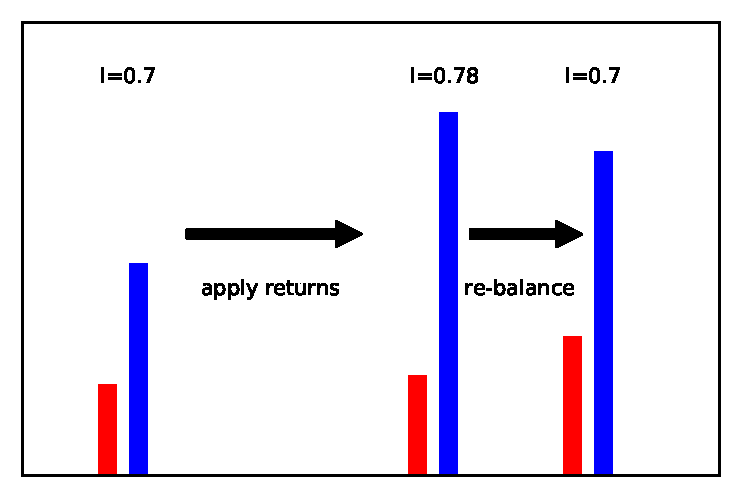
\includegraphics[width=\textwidth]{./chapter_4/figs/rebalance.pdf}
\caption{Investment in a risky (blue) and riskless (red) asset. Leverage starts at $\l=0.7$, meaning 70\% is invested in the risky asset, and 30\% in the riskless. The investment then experiences the relative returns of the market. In this case the riskless goes up a little, and the risky asset goes up more. Consequently, the leverage changes. To maintain a constent leverage, some risky asset has to be sold in return for some riskless, a step known as re-balancing.
\flabel{rebalance}}
\end{figure}
In the simplest instance, the overall effect is the following protocol 
\be
\xl(\t+\Dt;\l) = \underbrace{\rs(\t) \l \xl(\t;\l) }_{\text{new risky holdings}} + \underbrace{ \rr(\t)(1-\l) \xl(\t;\l)}_{\text{new bank deposits}},
\ee
which we repeat until the final day of the backtest, $\t_{\text{max}}$, when the final equity $\xl(\t_{\text{max}};\l)$ is recorded. 
\Fref{STR_trajectories} shows a few trajectories of leveraged investments in the S\&P500TR at different leverages $\l$.

\begin{figure}
\centering
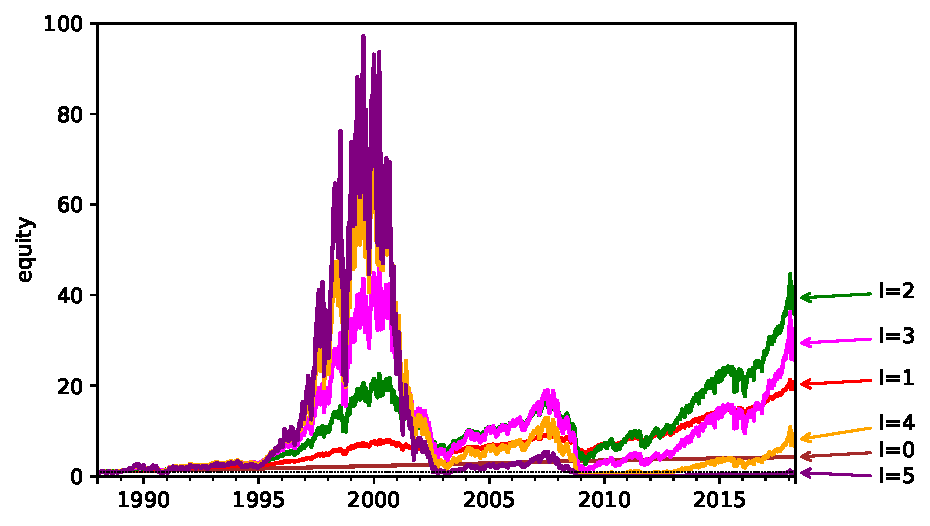
\includegraphics[width=\textwidth]{./chapter_4/figs/STR-FED-1_equity.pdf}
\caption{Equity $\xl(\t; \l)$ for investments of initially \$1 in the \SPT at different constant leverages, where money is borrowed at overnight federal interest rates. As leverage increases, eventually the fluctuations become harmful and the investor loses money. Each leverage produces one value for the final equity.
\flabel{STR_trajectories}}
\end{figure}

The procedure is then repeated for different leverages, and the optimal leverage is that which maximizes the final equity -- the trajectories $\xl(\t;\l)$ are turned into curves $\xl(\t_{\text{max}}; \l)$ by fixing $\t=\t_{\text{max}}$, see \fref{STR_final_equity}. 
If at any time the equity falls below zero, the investment is declared bankrupt and the backtest is considered invalid for the corresponding leverage. This happens when the leverage is very high and the risky asset dropped in value, or when it's very negative and the risky asset rises in value. Between these extremes, a smooth curve emerges, resembling an Gaussian bell-shape (or an upside-down parabola on logarithmic vertical scales).
\begin{figure}
\centering
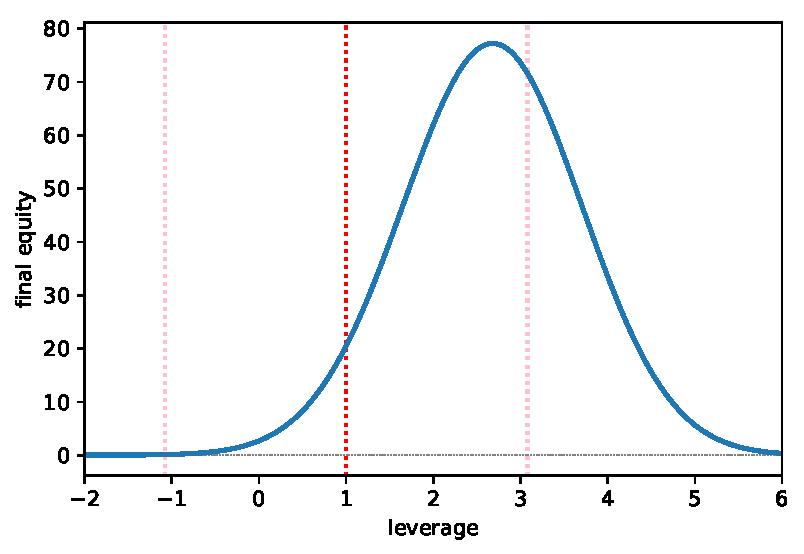
\includegraphics[width=\textwidth]{./chapter_4/figs/STR-FED_final_equity.pdf}
\caption{Final equity $\xl(\tn; \l)$ for investments of initially \$1 in the \SPT for 500 different leverages. These are the right-most end points of trajectories like in \fref{STR_trajectories}. The vertical lines indicate our best guess of the position of the optimum at $1$, and the range up to 2 standard errors away.
\flabel{STR_final_equity}}
\end{figure}

\FloatBarrier 
\subsubsection{Data sets}
We want to compare the true performance of one asset to that of another, and therefore it's important to find time series that really resemble changes in equity over time that an investment would have experienced. A stock market index would be nice because it will give a broad overall impression. It won't depend too much on the specific fortunes of any given company.

Strangely, most stock indexes are simply weighted averages of (free-float) market capitalization of a bunch of listed companies, but when one of those companies pays a dividend of \$10, and its shares correspondingly drop by \$10, the index drops too. We don't want that, so we'll have to find an index that properly accounts for dividends. The \SPT does that, so that we'll use that as one risky asset and play it against overnight federal deposits as the riskfree asset.

Another index that includes dividends is the German DAX, so we'll try that out too. In this case we will use German overnight deposits for the riskfree asset.

Bitcoin is another great asset to try out. It doesn't pay any dividends, so we don't have to worry about that, and its performance has been very different from that of a stock market, so it will be informative to see if leverage efficiency applies here too. 

Spoiler alert: bitcoin looks unremarkable from the point of view of leverage efficiency. Its volatility is just as predicted. But to understand the limitations of a model we have to push it beyond its range of applicability. We actually thought bitcoin would do the trick, but it didn't. So we'll use an asset that has officially been declared bullshit: investments in Bernie Madoff's ponzi scheme. Monthly returns were included in a now famous whistleblowing complaint to the \SEC. We took that complaint, digitized the returns and ran backtests as for the other assets.

For all assets, we will overestimate real optimal leverage in the most straight-forward backtest. Here are some reasons: 
\begin{enumerate}
\item Whenever trading occurs to rebalance the portfolio, trading costs would be incurred in reality. 
\item Money borrowed for leveraging up (and shares borrowed for shorting) come at a premium that the investor has to pay. 
\item Stock indexes reflect well diversified portfolios of successful companies -- they are affected by survivorship bias because unsuccessful companies leave the index. 
\item Overnight interest rates are very low. We use them because we want to have the possibility of accessing funds daily, but in real life that's not how one would invest cash.
\end{enumerate}
We could try to correct for this bias, and we have done that in \cite{PetersAdamou2011}. The necessary assumptions make the results more realistic but also more dependent on subjective guesses, so we'll just stick to the simplest case here and note that it will produce an over-estimate of $\lopt$.

\subsubsection{Full time series}
\Fref{STR_final_equity} shows the leverage-return curve for the \SPT. The optimal leverage is a little greater than 1, but still within 2 standard errors from the prediction. Without further ado, let's add to this figure the same curves for the DAX and Bitcoin, this time on logarithmic vertical scales to see a bit more structure, \fref{STR_final_all}.  
\begin{figure}
\centering
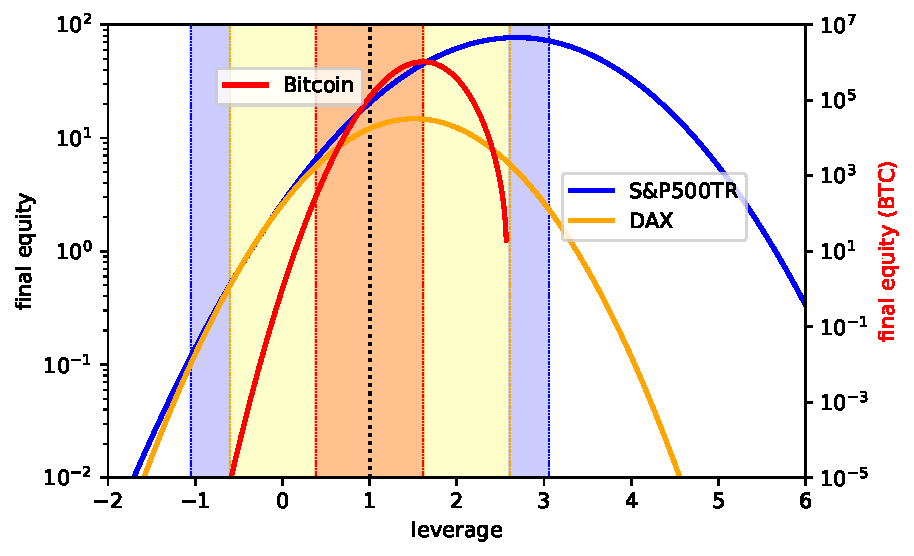
\includegraphics[width=\textwidth]{./chapter_4/figs/all_final_equity.pdf}
\caption{Final equity $\xl(\tn; \l)$ for investments of initially \$1 in the \SPT (blue), the DAX (yellow), and Bitcoin (red, scale on the right). The maxima of all three curves are near the predicted optimum of $\lopt=1$, where by ``near'' we mean that they are all within 2 standard errors of the prediction, see text.
\flabel{STR_final_all}}
\end{figure}

The overall impression that emerges is this: leverage efficiency is reasonably satisfied for these assets. The shaded areas in \fref{STR_final_all} show the predicted ranges, 2 statistical standard errors to the left and right from $\lopt=1$, and all observed maxima of the curves are within these bands. We also see a convincing bias: all estimates are greater than 1, as expected given the bias in the estimate that we mentioned earlier.

From a scientific point of view it's not very interesting to show lots of cases where a theory gives good predictions. We want to know the limits of the theory. When does it not apply? Where does it break down? To be honest, before we looked at the data we thought that bitcoin might be an example of an asset that doesn't obey leverage efficiency. But it looks unspectacular -- just as predicted. We didn't have a specific reason to suspect that the theory wouldn't apply to bitcoin, it just seemed like an extreme case that might not work for some reason. 

But let's see what happens where the theory really doesn't apply. In \fref{STR_final_all_MAD} we add to the curves of \fref{STR_final_all} the return-vs.-leverage curve for Bernie Madoff's fund. This is instructive because it shows just how different the results could have been. If it weren't for leverage efficiency optimal leverage for the \SPT, for example, could be miles away from our prediction. We have to show the Madoff data in a separate figure 
because the scales are so different that the differences between Bitcoin, \SPT, and the DAX become very small, and we thought they may be of interest.
Apart from showing the limits of our theory, the Madoff data suggest that leverage-return curves can help detect investments that are too good to be true, \ie fraud. 

Of course, Madoff could have chosen the invented returns of his fund in a way that's consistent with leverage efficiency, just to show the victims of his fraud something realistic. But apparently he didn't bother to do that, and people believed that he'd really found a way to print money.

That's good for us -- showing that a theory fails to predict things it shouldn't be able to predict is important. A theory about asset price fluctuations that applies even to ficitious prices like Madoff's would be suspicious -- it would probably not say much about prices at all but just be a statement that's generally true about a much broader class of phenomena. 
\begin{figure}
\centering
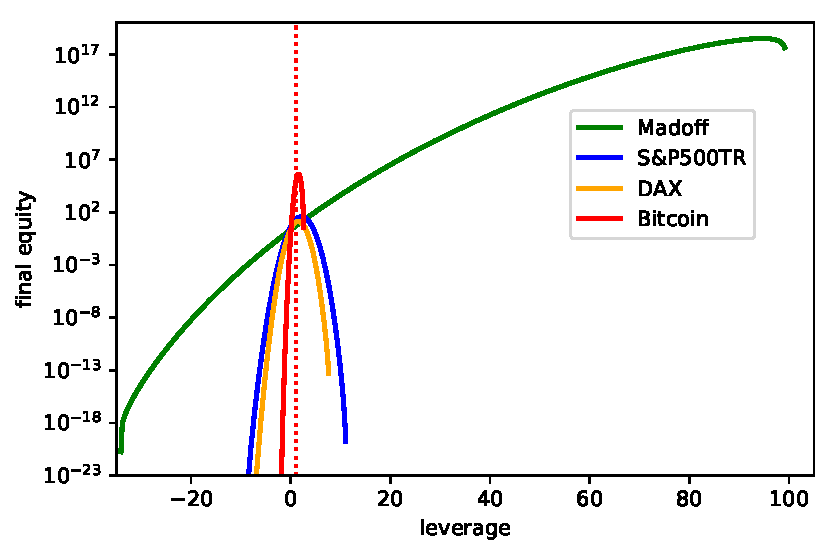
\includegraphics[width=\textwidth]{./chapter_4/figs/all_MAD_final_equity.pdf}
\caption{Final equity for investments of initially \$1 in the \SPT (blue), the DAX (yellow), Bitcoin (red), and Bernie Madoff's ponzi scheme. 
The maxima for the real assets cluster near the predicted value $\lopt=1$. Madoff's freely invented performance had such low volatility that a leverage of 100 would have been optimal, even if rebalancing could have only occurred once per month. At higher rebalancing frequencies (had the asset actually existed) the green curve would be seen to be the left end of a parabola whose maximum may well be at 200 or 300.
\flabel{STR_final_all_MAD}}
\end{figure}

\subsubsection{Shorter time scales}
In \secref{Prediction_accuracy} we derived an expression, \eref{variance}, for the variance of optimal leverage that we expect to observe in a finite time series, and we used this to arrive at a statistical error estimate, a scale on which to judge whether leverage efficiency holds or not.
But we can use \eref{variance} as a prediction in itself: is the sample variance of $\lopt$, measured in many windows of size $\Dt$ well described by \eref{variance}? While we can't make the time series longer than they are, we can make the shorter and collect statistics over non-overlapping windows. \Fref{loglog} shows the result.
%\fref{g_l_linear} shows the simulated multiplicative return as a function of leverage for an investment over the entire time series.
%\begin{figure}
%\centering
%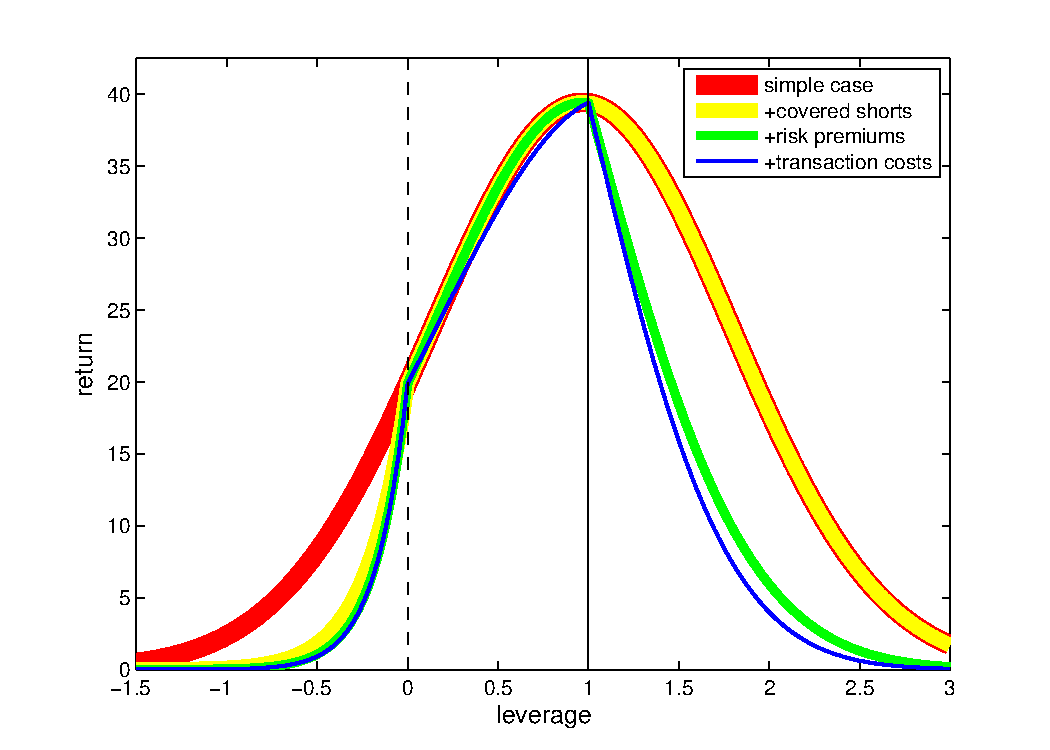
\includegraphics[width=\textwidth]{./chapter_4/figs/sme_fig1.pdf}
%\caption{Total return for a constant-leverage investment in the S\&P500, starting $4^{\text{th}}$ August 1955 and ending $21^{\text{st}}$ May 2013 as a function of the leverage.
%\newline \underline{Red line:} Simulation 1. Interest at federal funds rate on bank deposits and loans. No stock borrowing costs. No transaction costs.
%\newline \underline{Yellow line:} Simulation 2. As 1, but with interest at federal funds rate on borrowed stock. This introduces a kink at $\l=0$, where stock borrowing begins.
%\newline \underline{Green line:}\ Simulation 3. As 2, but with interest charged at the higher bank prime rate on borrowed cash and stock. This introduces a kink at $\l=1$.
%\newline \underline{Blue line:}\ Simulation 4. As 3, but with a transaction cost of 0.2\% of the value of the assets traded on rebalancing.\flabel{g_l_linear}}
%\end{figure}
%The four curves in the figure correspond to four sets of assumptions about interest rates and transaction costs. These are labelled 1--4 in order of increasing complexity and resemblance to actual practices in financial markets. We will not dwell on these here, although brief descriptions are provided in the figure caption.
%
%$\lopt=0.97$ for simulations 1 (which we will refer to as the simple case), 2, and 3. $\lopt=1.00$ for the most realistic simulation, 4 (the complex case). These results appear to lend great support to the stochastic market efficiency hypothesis. Based on simple thought experiments motivated by the theories developed in these lectures, we predicted that $\lopt$ in a real market should be close to unity. 58 years of real market data confirm this prediction. We discuss below the statistical significance of these results.
%
%The kinks\footnote{A non-technical term for discontinuities in the derivative.} in the return-leverage curve can be accompanied by a change in sign of the derivative. When this happens, the kink is a global maximum and $\lopt$ is fixed at that leverage, either 0 or 1. This makes these special leverages sticky, in that $\lopt$ can get trapped there.\footnote{Although typically only when the $\lopt$ of simulation 1 is already in or very close to the range, $0\leq\lopt\leq1$.}. This stickiness will tend to promote the likelihood of the hypothesis being confirmed. However, simulation 1 shows that $\lopt\approx1$ even when these effects are neglected.
%
%\textbf{Parameter estimation}\\
%\fref{g_l_logarithmic} shows the simulated growth rate as a function of leverage for the simple case (simulation 1) over the entire time series.
%\begin{figure}
%\centering
%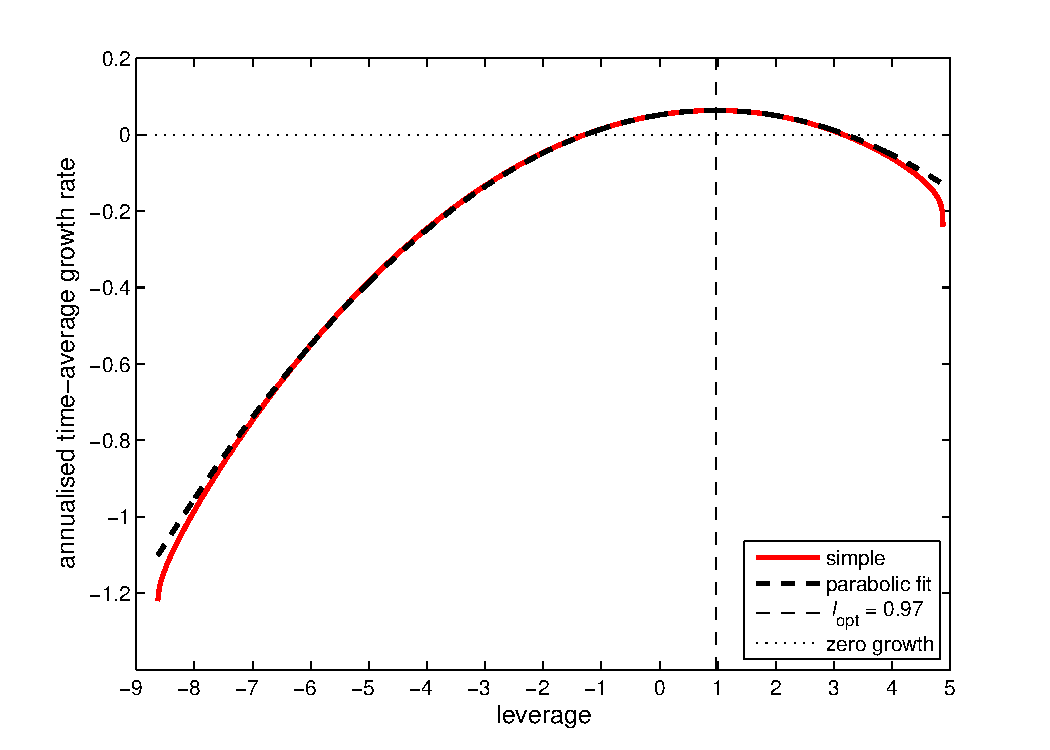
\includegraphics[width=\textwidth]{./chapter_4/figs/sme_fig2.pdf}
%\caption{Computed time-average growth rates closely follow a parabola as a function of leverage.\flabel{g_l_logarithmic}}
%\end{figure}
%This is the logarithm of the simulated return of \fref{g_l_linear} divided by the window length. Since the window is long, we might expect to approximate the time-average growth rate, $\gtm(\l)$, which we know from \eref{g_l_quadratic} is a parabola in the original \GBM model. The black dashed line is a fitted parabola, whose parameters can be taken as meaningful definitions of the effective values of $\mur$, $\mue$, and $\sigmas$ for the S\&P500 for the entire time series.\footnote{We say effective because, although we think of these parameters as being time-varying in the relaxed model, their values from the parabolic fit are those of the original constant-parameter model which produce an almost identical outcome for $\gtm(\l)$ as the real data.} A least-squares fit estimates these parameters as $\mur=5.2\%$ \textit{pa}, $\mue=2.4\%$ \textit{pa}, and $\sigmas=16\%$ \textit{p$\sqrt{\mathit{a}}$}.
%
%The deviation from parabolic form for high and low leverages in \fref{g_l_logarithmic} is due to extremely large fluctuations in the index, which are much less rare than would be observed in a true \GBM. These result in large losses and, indeed, bankruptcy for highly leveraged portfolios. That real returns distributions are observed to have fatter tails than those predicted by \GBM is an oft-made criticism of classical theory. In this study it is not especially relevant: indeed, the existence of rogue fluctuations strengthens the stochastic efficiency hypothesis, in that it penalises high leverage strategies.
%
%\textbf{Finite time scales}\\
%In the real world, of course, we can never truly observe the time-average growth rate of a leveraged investment since this would require an infinite observation time. Instead we observe the finite-time growth rate over a window of length $\Dt$. This is a random variable whose distribution broadens as $\Dt\to0$
%
%Likewise, we never truly observe $\lopt$ either, since this is the leverage that maximises a time average-growth rate. Instead we observe simulated optimal leverages which maximise finite-time growth rates. We can guess that these will show larger fluctuations from the underlying $\lopt$ as the simulation window gets shorter, because short periods containing a sequence of almost all positive or negative stock price movements will result in very high (possibly infinite) positive or negative simulated optimal leverages.
%
%More formally, let's denote by $\loptc(\Dt)$ the simulated optimal leverage which maximises the finite-time growth rate, $\gm(\xl,\Dt)$. As $\Dt\to0$, $\gm(\xl,\Dt)$ becomes a worse estimator of the time-average growth rate, $\gtm(\l)$, because its distribution becomes broader. Thus $\loptc(\Dt)$ becomes a similarly worse estimator of $\lopt$. 
%
%This is important because a single observation of $\loptc(\Dt)$ consistent with our hypothesis (such as the one we just made for $\Dt\approx58$ years) is only significant if the uncertainty in $\loptc(\Dt)$ is of the same order of magnitude as $\loptc(\Dt)$ itself. For example, if we knew that $\loptc(\Dt)$ had a distribution that could place it between, say, -10 and 10 with reasonable probability, then we couldn't read much from a single observation either inside or outside the attractive range of our hypothesis. If, on the other hand, most of the distribution's mass were inside the range, then an observation outside would be strong evidence that the hypothesis is flawed, and so an observation inside is significant.
%
%We can quantify these ideas in the original model by discarding the $\Dt\to\infty$ limit in \eref{g_l_noisy}. This gives
%\be
%\gm(\xl,\Dt) = \mur+\l\mue-\frac{\l^2\sigmas^2}{2}+\frac{\l\sigmas \gW(\Dt)}{\Dt},
%\elabel{g_l_finite}
%\ee
%which is maximised at
%\be
%\loptc(\Dt) = \lopt + \frac{\gW(\Dt)}{\sigmas\Dt}.
%\elabel{lopt_finite}
%\ee
%This is normally distributed with mean $\lopt$ and standard deviation
%\be
%\text{stdev}[\loptc(\Dt)] = \frac{1}{\sigmas\sqrt{\Dt}}.
%\elabel{lopt_sd}
%\ee
%Using the computed volatility of $16\%$ per square root of one year, this standard deviation is approximately 0.83. This means that the uncertainty in $\loptc(\Dt)$ is about the same size as the hypothesised value of $\lopt$, and so the single observation we made is a significant corroboration of the hypothesis.
%
%We can also test the validity of the relationship in \eref{lopt_finite} by simulating investments of different window lengths in the market data and compiling histograms of the resulting $\loptc(\Dt)$. \fref{loglog} shows, on double-logarithmic scales, the standard deviation of $\loptc(\Dt)$ as a function of $\Dt$ for the simple simulation.
\begin{figure}
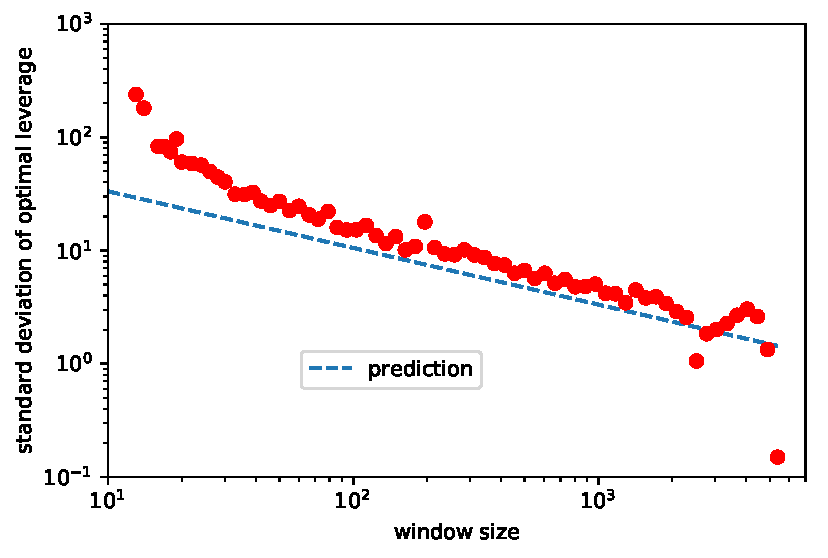
\includegraphics[width=\textwidth]{./chapter_4/figs/STR-FED_lopt_var.pdf}
\caption{The red dots show the standard deviation of samples of $\loptc(\Dt)$ as a function of window length measured in days. The blue dashed line shows the prediction of \eref{variance} using the estimate of $\sigmas$ obtained by fitting a parabola to the \SPT curve in \fref{STR_final_all}.\flabel{loglog}}
\end{figure}

Good agreement is found with the model-specific prediction. The structure we have identified -- leverage efficiency -- operates on all time scales from weeks to decades. This broad range of applicability supports our theory of noise in \secref{a_theory}: it is a requirement of stability that asset prices fluctuate, and the shorter the time scales the less significant any economic information becomes. Thinking of price changes as a reflection of the arrival of new information is simply the wrong starting point. Artificially suppressing fluctuations destabilizes the financial system -- observations of assets whose prices don't flucutate sufficiently indicate bubbles being inflated.

%\footnote{For shorter time scales, the standard deviation is slightly higher than predicted. We suspect this is due to discretisation effects: for investments over a small number of days, very high optimal leverages can be observed when the window contains predominantly positive or negative index movements. These would no longer be optimal if fluctuations and rebalancing were simulated on smaller time scales, \ie intra-day. For longer time scales, the standard deviation drops below the prediction. This is because for window lengths approaching the entire period under study, the number of independent windows in the sample is small, and so the standard deviation of the sample is depressed.}
%
%\fref{l_opt_expanding} shows the simulated $\loptc(\Dt)$ for the investment window starting on $4^\text{th}$ August 1955 and ending on the date on the horizontal axis.
%\begin{figure}
%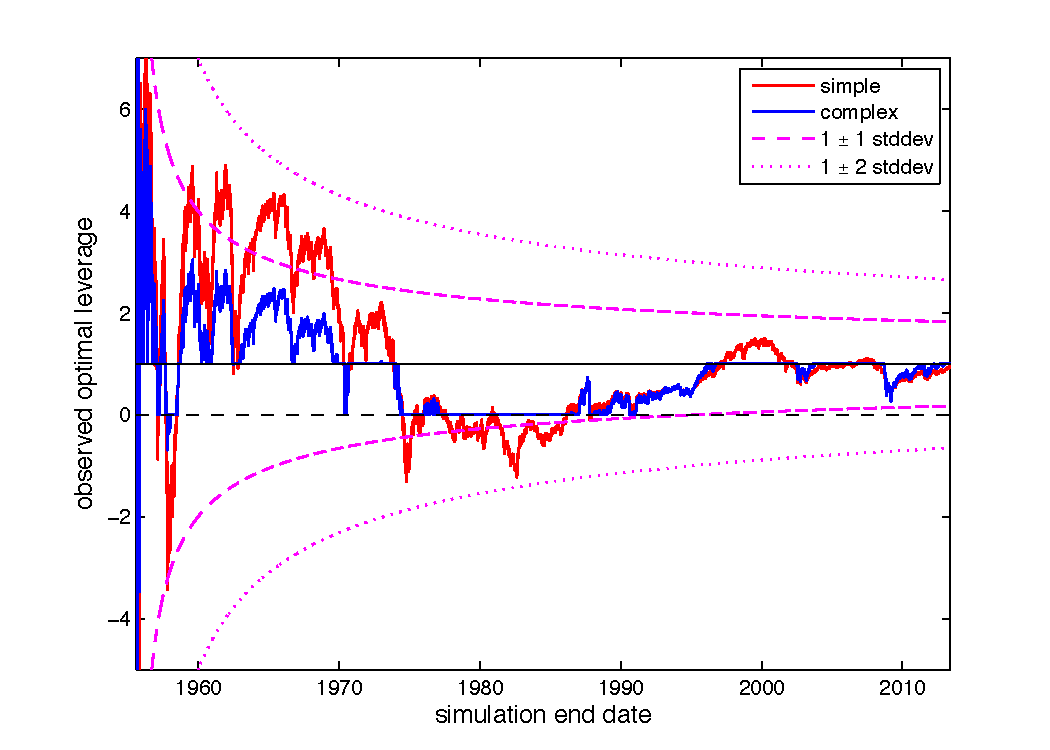
\includegraphics[width=\textwidth]{./chapter_4/figs/sme_fig4.pdf}
%\caption{Daily simulated optimal leverages for an expanding window with start date $4^\text{th}$ August 1955 and end date on the horizontal axis. Both simple (red line) and complex (blue line) simulations are shown. The broken magenta lines show the one- and two-standard deviation envelopes about $\lopt=1$, based on \eref{lopt_sd} and the estimate of $\sigmas$ from the parabolic fit in \fref{g_l_logarithmic}.\flabel{l_opt_expanding}}
%\end{figure}
%The reduction in fluctuations with increasing window length are broadly consistent with \eref{lopt_sd} and support the hypothesis that $\lopt$ -- as estimated by $\loptc(\Dt)$ -- is attracted to the range $0\leq\lopt\leq1$ and, over long time scales, to $\lopt=1$ in particular.
%
%We can also plot the simulated optimal leverages for investment windows with fixed lengths and moving start date. We do this for the simple and complex simulations in \fref{l_opt_expanding}, with window lengths ranging from 5 to 40 years.
%\begin{figure}
%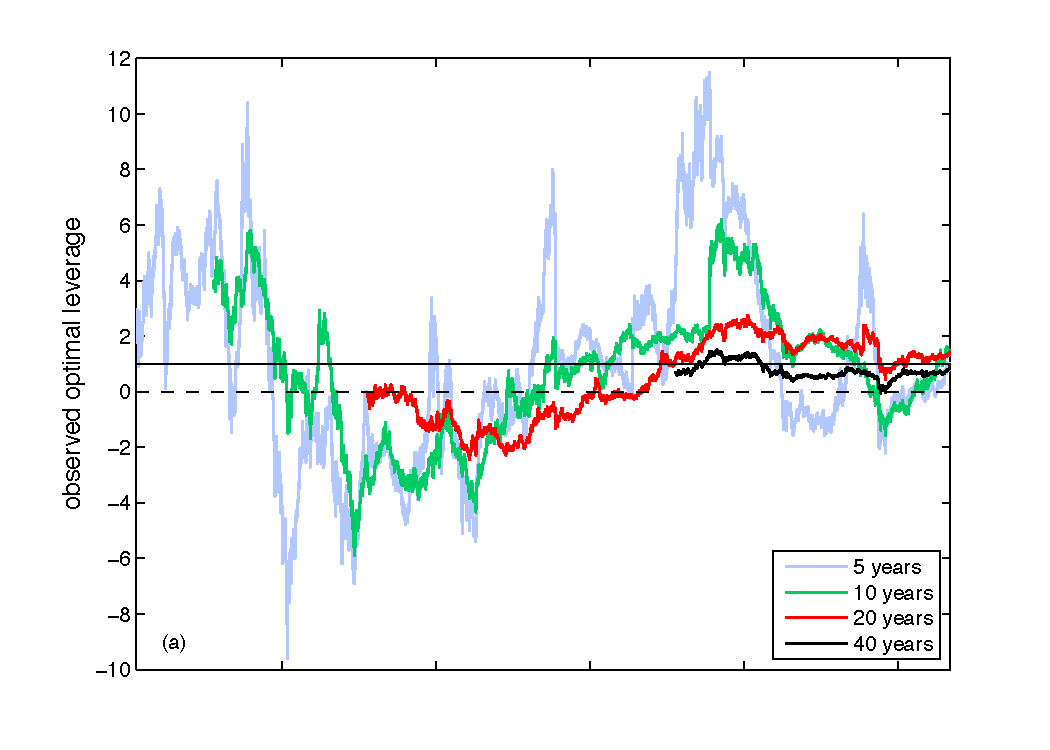
\includegraphics[width=1.\textwidth]{./chapter_4/figs/sme_fig5a.pdf}
%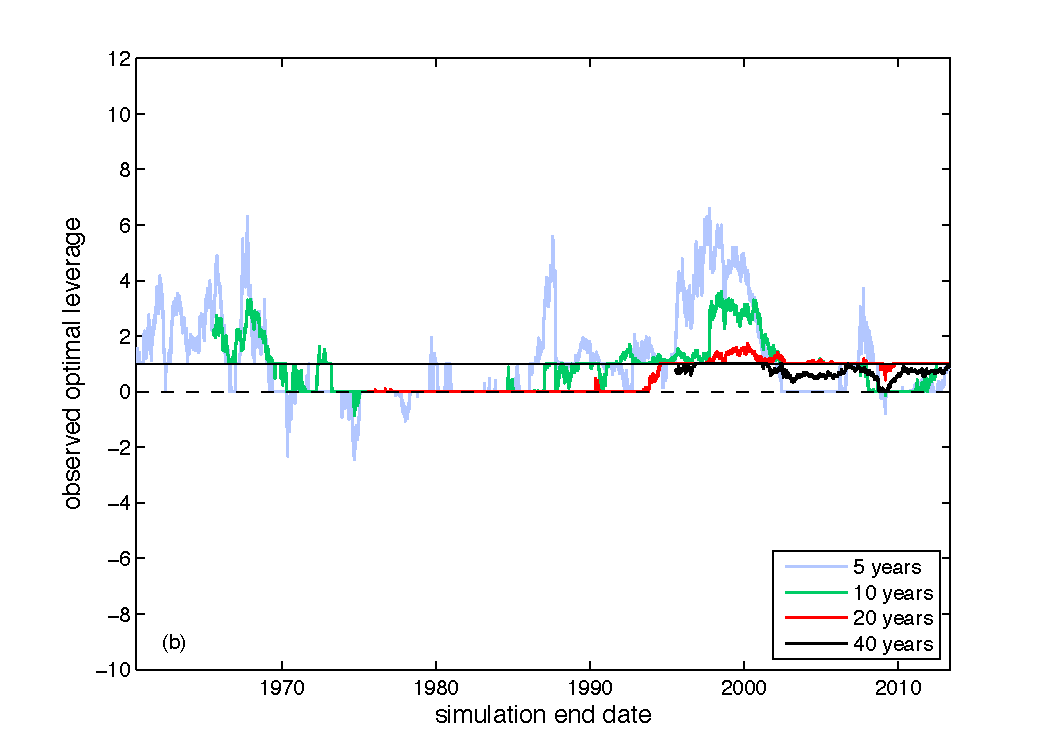
\includegraphics[width=1.\textwidth]{./chapter_4/figs/sme_fig5b.pdf}
%\caption{\newline
%(a) In the simple simulation, observed optimal leverage fluctuates strongly on short time scales but appears to converge to $\loptc(\Dt)=1$ on long time scales. This constitutes the central result of the study.
%\newline
%(b) In the complex simulation, the kinks in \fref{g_l_linear} ensure that $\loptc(\Dt)=0,1$ are often found exactly. The 40-year simulation supports the strong stochastic efficiency hypothesis, that real markets are attracted to $\lopt=1$, with a dip to $\lopt=0$ only during the financial crisis of 2008. \flabel{l_opt_fixed}}
%\end{figure}
%From the strong fluctuations over short time scales emerges attractive behaviour consistent with our refined hypothesis. The effects of the stickiness of the points $\lopt=0$ and $\lopt=1$ in the complex model are clearly visible. In particular, over the last decade or so optimal leverage for the 20- and 40-year windows remained close to unity.
%
%
%%%%%%%%%%%%%%%%%%%%%%%%%%%%%%%%%%%%%%%%%%%%%%%%
%
%%%%%%%%%%%%%%%%%%%%%%%%%%%%%%%%%%%%%%%%%%%%%%%%
\subsection{Discussion}
The primary aim of this final lecture was to demonstrate that the mathematical formalism we have developed to conceptualise randomness in economics, which started with a simple model of wealth evolution by repetition of a gamble, is very powerful. It does more than simply create a rigorous and plausible foundation for economic theory. In particular, because the framework is epistemologically sound, we can make testable predictions -- such as the stochastic market efficiency hypothesis -- which we can corroborate empirically using real economic data. We could not have guessed from our simple coin-tossing game that we would end up making a prediction about the fluctuations of the American stock market or those of bitcoin. What other surprising predictions can we make in this formalism? That, dear reader, is a question for you.

%%%%%%%%%%%%%%%%%%%%%%%%%%%%%%%%%%%%%%%%%%%%%%%
